% JoonHo Lee (jlee296@ua.edu)
% The published needs-review workflow and official rating hierarchy.
\documentclass[border=4pt]{standalone}
\usepackage[T1]{fontenc}
\usepackage{helvet}
\renewcommand{\familydefault}{\sfdefault}
\usepackage{tikz}
\usetikzlibrary{positioning, arrows.meta, calc, fit, backgrounds}
\usepackage{xcolor}
\definecolor{lanegrey}{HTML}{E7EDF2}
\definecolor{laneedge}{HTML}{6E8CA0}
\definecolor{propfill}{HTML}{EFE9F4}
\definecolor{propedge}{HTML}{7A5A9A}
\definecolor{propink}{HTML}{3F007D}
\definecolor{ink}{HTML}{20303C}
\definecolor{muted}{HTML}{5A6B78}
\pdfinfo{/Author (JoonHo Lee (jlee296@ua.edu)) /Title (Needs review and the CDBG application process)}
\begin{document}
\hyphenpenalty=10000\exhyphenpenalty=10000
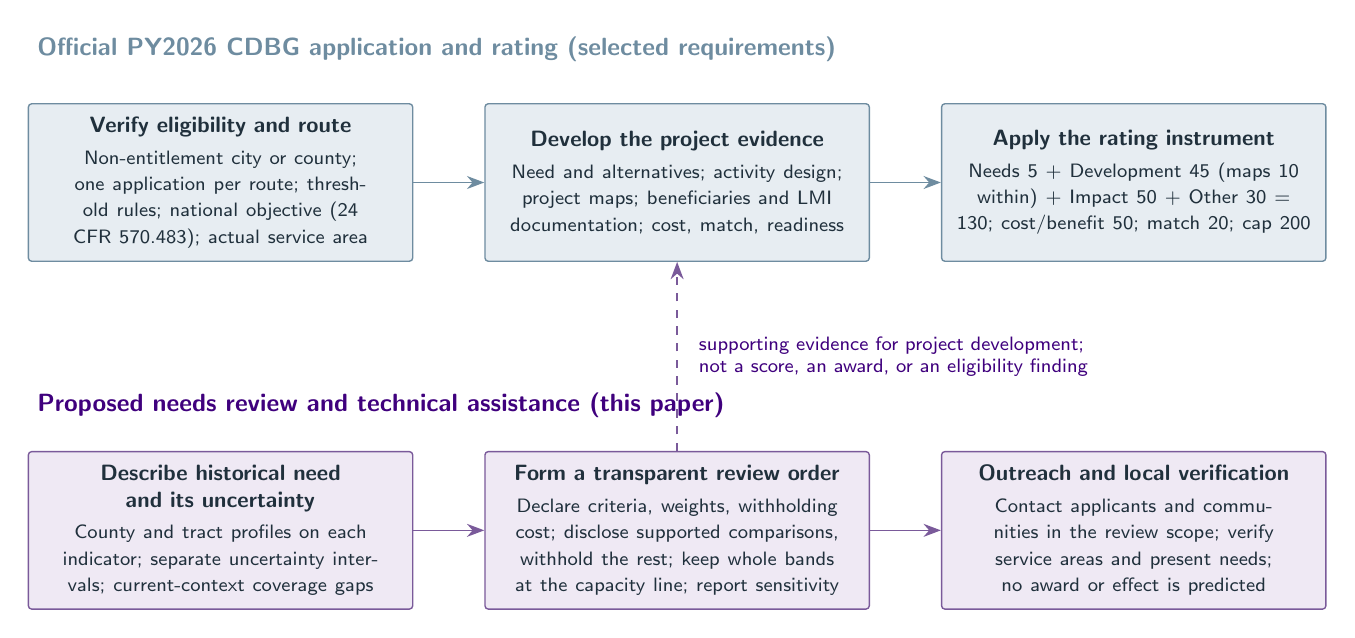
\begin{tikzpicture}[
  font=\footnotesize, >={Stealth[length=2.2mm]},
  box/.style={draw, line width=0.5pt, rounded corners=1.2pt, align=center, inner sep=4pt, text width=46mm, minimum height=20mm, text=ink},
  official/.style={box, fill=lanegrey, draw=laneedge},
  proposed/.style={box, fill=propfill, draw=propedge},
  title/.style={font=\footnotesize\bfseries},
  body/.style={font=\scriptsize, text=ink},
  lane/.style={font=\small\bfseries},
  arrow/.style={->, line width=0.6pt, draw=laneedge},
  parrow/.style={->, line width=0.6pt, draw=propedge},
  flow/.style={->, line width=0.6pt, draw=propedge, dashed}]

% ---- official lane -------------------------------------------------------------------
\node[official] (o1) {\textbf{Verify eligibility and route}\\[2pt] \scriptsize Non-entitlement city or county; one application per route; threshold rules; national objective (24 CFR 570.483); actual service area};
\node[official, right=9mm of o1] (o2) {\textbf{Develop the project evidence}\\[2pt] \scriptsize Need and alternatives; activity design; project maps; beneficiaries and LMI documentation; cost, match, readiness};
\node[official, right=9mm of o2] (o3) {\textbf{Apply the rating instrument}\\[2pt] \scriptsize Needs 5 + Development 45 (maps 10 within) + Impact 50 + Other 30 = 130; cost/benefit 50; match 20; cap 200};
\draw[arrow] (o1) -- (o2); \draw[arrow] (o2) -- (o3);
\node[lane, text=laneedge, above=4mm of o1.north west, anchor=south west] (olabel) {Official PY2026 CDBG application and rating (selected requirements)};

% ---- proposed lane -------------------------------------------------------------------
\node[proposed, below=24mm of o1] (r1) {\textbf{Describe historical need and its uncertainty}\\[2pt] \scriptsize County and tract profiles on each indicator; separate uncertainty intervals; current-context coverage gaps};
\node[proposed, right=9mm of r1] (r2) {\textbf{Form a transparent review order}\\[2pt] \scriptsize Declare criteria, weights, withholding cost; disclose supported comparisons, withhold the rest; keep whole bands at the capacity line; report sensitivity};
\node[proposed, right=9mm of r2] (r3) {\textbf{Outreach and local verification}\\[2pt] \scriptsize Contact applicants and communities in the review scope; verify service areas and present needs; no award or effect is predicted};
\draw[parrow] (r1) -- (r2); \draw[parrow] (r2) -- (r3);
\node[lane, text=propink, above=3mm of r1.north west, anchor=south west] (rlabel) {Proposed needs review and technical assistance (this paper)};

% ---- connection -----------------------------------------------------------------------
\draw[flow] (r2.north) -- node[right=1.5mm, align=left, font=\scriptsize, text=propink] {supporting evidence for project development;\\ not a score, an award, or an eligibility finding} (o2.south);

\end{tikzpicture}
\end{document}
